%#######################################################################
% English task description for task "cache"
%
% Copyright (C): 2019, HAUER Daniel, daniel.hauer@tuwien.ac.at
% License GPL V2 or later (see http://www.gnu.org/licenses/gpl2.txt)
%#######################################################################

\documentclass[a4paper,12pt]{article}
\usepackage{a4wide}
\usepackage{tikz}
\usetikzlibrary{calc}
\usepackage[ngerman]{babel}

\begin{document}
\pagestyle{empty}
\setlength{\parindent}{0em} 
\section*{\noindent Cache }

Your task is to program the behavior of an entity called "cache". This entity is declared in the attached file "cache.vhdl" and has the following properties:


\begin{itemize}
	\item Input: addr with type std\_logic\_vector of length {{addr_length}}
	\item Input: en\_read with type std\_logic
	\item Input: clk with type std\_logic
	\item Output: data with type std\_logic\_vector of length {{data_length}}
	\item Output: ch\_cm with type std\_logic

\end{itemize}

\begin{center}
\begin{tikzpicture}
\draw node [draw,rectangle, minimum height=24mm, minimum width=35mm,rounded corners=2mm,thick](entity){};

\draw[->] ($ (entity.west)+(-10mm,6.0mm)$) -- ($ (entity.west) + (0mm,6.0mm)$);
\draw[anchor=east] node at ($ (entity.west)+(-9mm,6.0mm)$){ addr };

\draw[->] ($ (entity.west)+(-10mm,0.0mm)$) -- ($ (entity.west) + (0mm,0.0mm)$);
\draw[anchor=east] node at ($ (entity.west)+(-9mm,0.0mm)$){ en\_read };

\draw[->] ($ (entity.west)+(-10mm,-6.0mm)$) -- ($ (entity.west) + (0mm,-6.0mm)$);
\draw[anchor=east] node at ($ (entity.west)+(-9mm,-6.0mm)$){ clk };


\draw[->] ($ (entity.east) + (0mm,4.0mm)$) -- ($ (entity.east) + (10mm,4.0mm)$);
\draw[anchor=west] node at ($ (entity.east) + (9mm,4.0mm)$){ data };

\draw[->] ($ (entity.east) + (0mm,-4.0mm)$) -- ($ (entity.east) + (10mm,-4.0mm)$);
\draw[anchor=west] node at ($ (entity.east) + (9mm,-4.0mm)$){ ch\_cm };


\draw node at ($ (entity) - (0,0mm)$){ cache };

\end{tikzpicture}
\end{center}

Do not change the file "cache.vhdl"!\\

The aim of this task is to program the reading unit of a \textit{direct mapped} cache. Depending on the address set at the address input \textit{addr}, the cache has to be searched and the memory content has to be returned in case of a \textit{cache hit}. With a \textit{direct mapped cache}, the position of a date in the cache is uniquely defined by the address. If the cache contains M entries, then N = $\lceil log_2(M) \rceil$ bits of the address are required for the position calculation (= index) in the cache and the remaining bits of the address are additionally stored in the cache as a \textit{tag}.
When checking whether a date exists in the cache, the position in the cache must first be calculated using a part of the address and then the stored \textit{tag} must be compared with the second part of the address. If this matches, a \textit{cache hit} is detected. Figure \ref{img_cache} illustrates the concept of a direct mapped cache.
 

\begin{figure}[h]
\begin{center}
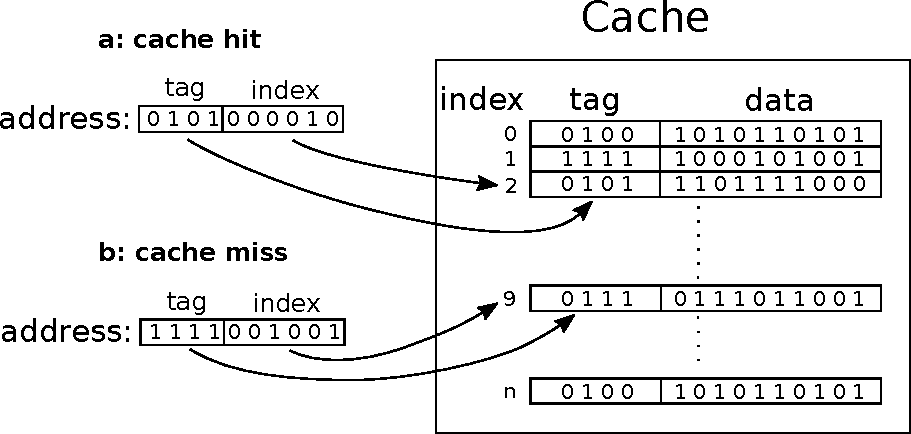
\includegraphics[width=0.75\textwidth]{../static/cache.pdf}
\caption{Principle of read access for a \textit{direct mapped} cache. In the figure you can see an example for a \textit{cache hit} (a) and a \textit{cache miss} (b). \newline (Attention: The bit widths used in this example do not necessarily correspond to the bit width of your specific task description.)}
\label{img_cache}
\end{center}
\end{figure}

The "cache" entity shall behave according to the following:\\

\begin{itemize}

\item The cache shall operate on

falling

rising

 edges of the clock input\textit{clk}. Therefore the outputs shall only change on a

falling

rising

edge.

\item The cache is only accessible if \textit{en\_read} is ' 1', otherwise the output \textit{data} should always be High Impedance ('Z') and the flag \textit{ch\_cm} should always return '0'.

\item The {{cache_size}} entries stored in the cache and its tags are given in table \ref{tab_cachedata} and should be set as constant content in your cache. (This would normaly be done by the writing unit of the cache.)

\item If a read access occurs (\textit{en\_read} = '1'), the potential position of the data in the cache (= index) and the related tag should be calculated from the address \textit{addr}. If a \textit{cache hit} occurs, the data at this address should be output at the output \textit{data} and the flag \textit{ch\_cm} set to '1'. If a \textit{cache miss} occurs, the output \textit{data}  should set to High Impedance ('Z') and the flag \textit{ch\_cm} set to '0'. 


\item If during a read access the cache index of the address is greater than the memory depth of the cache, the output \textit{data}  should also be High Impedance ('Z') and the flag \textit{ch\_cm} should return '0'.

\item For the calculation of the cache index and the tag from the given address, you have to consider the following: The index is calculated from the n least significant address bits, where n is the minimum number of bits required to display all {{cache_size}} indices in the cache. The remaining m bits are stored as tag (n + m = address length = {{addr_length}}). 


\end{itemize}

\begin{table}
\centering
\begin{tabular}{|c|c|c|}
\hline
~Cache Index~ & ~~~Tag~~~ & ~~~Data~~~ \\
\hline

{{i}}   & {{tag_values[i]}} & {{data_values[i]}} \\

\hline
\end{tabular}

\caption{Inhalt des Caches. Die Daten und Tags sind jeweils mit MSB first angegeben.}
\label{tab_cachedata}
\end{table}

This behavior has to be programmed in the attached file "cache\_beh.vhdl".\\

To turn in your solution, write an email to {{SUBMISSIONEMAIL}} with Subject "Result Task {{TASKNR}}" and attach your file "cache\_beh.vhdl".

\vspace{0.7cm}

Good Luck and May the Force be with you.
\end{document}
